\documentclass[a4paper]{article}

\usepackage[utf8]{inputenc}
\usepackage[T1]{fontenc}
\usepackage{textcomp}
\usepackage[italian]{babel}
\usepackage{amsmath, amssymb}
\usepackage{siunitx}
\usepackage{caption}
\usepackage{graphicx}
\usepackage{subcaption}
\usepackage{booktabs} % Opzionale, per tabelle più belle se vuoi (\toprule, \midrule, \bottomrule)
\usepackage{ragged2e} % Per \Centering nelle minipage
\usepackage{float} % Per [htbp]
\usepackage{fullwidth}
%\usepackage{darkmode} % Disabilitato come nell'originale
%\enabledarkmode
\usepackage[margin=2cm]{geometry}

% ======================================================
% Impostazioni siunitx (opzionale, ma utile)
% ======================================================
\sisetup{
    output-decimal-marker = {,}, % Usa la virgola come separatore decimale
    uncertainty-mode = separate, % Mostra incertezza come ±
    separate-uncertainty = true, % Forza la separazione
    locale = IT, % Impostazioni locali italiane (es. per la virgola)
    group-digits = false, % Evita di raggruppare le cifre (es. 10000 vs 10 000)
    per-mode=symbol % usa / per le unità composte es. km/h
}

% ======================================================
% Appendice con le tabelle dati
% ======================================================
\usepackage{titling}
\usepackage{appendix}
\usepackage[colorlinks=true, linkcolor=blue, citecolor=blue, urlcolor=blue]{hyperref} % Per riferimenti cliccabili (opzionale ma utile)
\usepackage[italian,nameinlink]{cleveref} % Per riferimenti più intelligenti (\cref, \Cref)

\renewcommand{\appendixname}{Appendice} % Traduce "Appendix" in "Appendice"
\renewcommand{\appendixtocname}{Appendici} % Traduce "Appendices" nel ToC
\renewcommand{\appendixpagename}{Appendici} % Traduce "Appendices" nell'header/footer

% Configurazioni cleveref per l'italiano
\crefname{section}{sezione}{sezioni}
\Crefname{section}{Sezione}{Sezioni}
\crefname{table}{tabella}{tabelle}
\Crefname{table}{Tabella}{Tabelle}
\crefname{figure}{figura}{figure}
\Crefname{figure}{Figura}{Figure}
\crefname{equation}{equazione}{equazioni}
\Crefname{equation}{Equazione}{Equazioni}
\crefname{footnote}{nota}{note}
\Crefname{footnote}{Nota}{Note}


\title{Interferometro}
\author{Alessio Ramirez, Michele Rota, Sofia Zocchi}
\date{Giugno 2025}


\begin{document}
\maketitle
\tableofcontents

\section{Interferometro di Fabry-Perot}
\subsection{Obiettivo}
Verificare la legge che descrive la posizione dei massimi di interferenza per la configurazione di Fabry-Perot

\subsection{Metodo}

\begin{figure}[htbp]
\centering
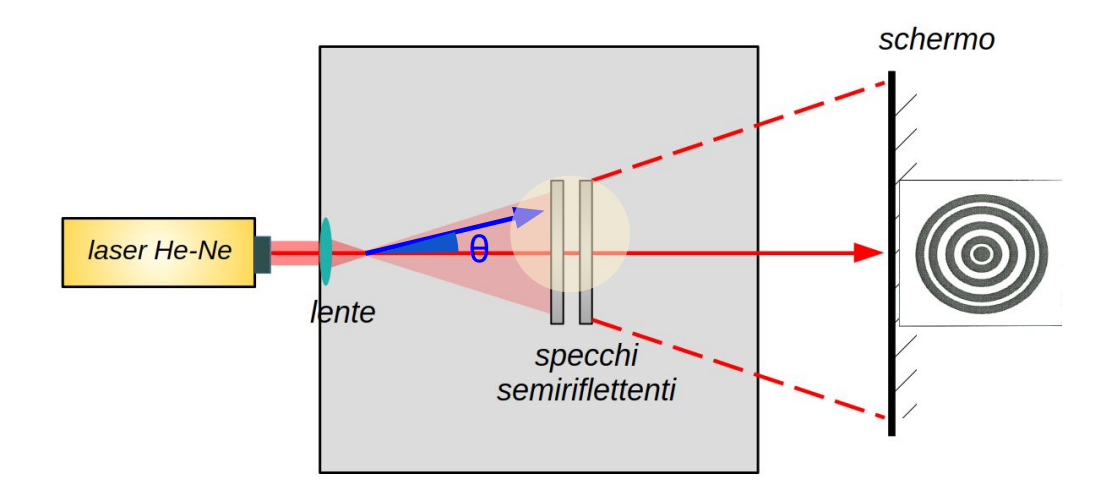
\includegraphics[width=1.0\textwidth]{./grafici/fabry_perot_immagine}
\caption{Schema interferometro di Fabry Perot}
\label{fig:fabry-perot-schema}
\end{figure}
Nella configurazione di Fabry-Perot, il laser emesso, che passa per una lente divergente, viene parzialmente riflesso nella cavità formata da due specchi paralleli e conseguentemente si hanno cammini ottici differenti per i raggi riflessi e trasmessi. 

Come schematizzato in figura \ref{fig:fabry-perot-schema} l'interferometro di Fabry-Perot è costituito da due superfici riflettenti parallele separate da una distanza $d$ regolabile. Il fascio laser incidente viene parzialmente riflesso e trasmesso quando incontra ogni parete della cavità, generando multiple riflessioni all'interno di quest'ultima. I raggi che emergono dalla cavità interferiscono tra loro, producendo una figura di interferenza.
Come lunghezza d'onda $\lambda$ del fascio laser abbiamo calcolato $\lambda = \frac{\lambda_0}{n}$, con $n=1.00029$ indice di rifrazione dell'aria e $\lambda_0 = 632.8$ come indicato sul manuale PASCO. Tramite questo passaggio abbiamo potuto tenere conto del fatto che la propagazione del laser non è avvenuta nel vuoto ma in aria, con conseguente variazione del suo reale cammino ottico.
Si può ricavare che la condizione per l'interferenza costruttiva è data dalla relazione:
\begin{align}
   \delta_r\frac{\lambda}{2\pi}+ 2d \cos \theta = N\lambda
\label{eq: max interferenza fabry-perot}
\end{align}
dove $d$ è la distanza tra gli specchi, $\theta$ è l'angolo di incidenza del raggio rispetto alla normale allo schermo, $N$ è un intero che indica l'ordine del massimo e $\lambda$ è la lunghezza d'onda della luce.

Il termine $\delta_r\frac{\lambda}{2\pi}$ tiene invece conto dello sfasamento dovuto dalle riflessioni multiple del secondo raggio (quello che non fuoriesce immediatamente dalla cavità).

Per verificare questa legge, sono stati misurati i diametri dei massimi di interferenza proiettati sulla parete, per diversi ordini di massimi, ed è stata misurata la distanza $L$ tra la lente \footnote{In quanto la lente è responsabile dell'apertura del fascio collimato (luce laser) essa può essere considerata come sorgente puntiforme a partire da cui si originano i raggi che andranno poi a interagire all'interno della cavità} e la parete. A partire da queste misure si è ricavato l'angolo $\theta$ con la seguente relazione:
\[\theta = \arctan \left(\frac{\text{diametro}}{2L}\right)\]

\subsection{Dati}
La distanza tra lente e parete, rimasta fissa per tutte le misure, è stata misurata come $L=\SI{128 \pm 0.5}{\centi\meter}$, mentre le misure dei vari diametri, e i relativi valori di $\cos{\theta}$ sono riportati in tabella \ref{tab:fabry-perot-dati}. Da notare come al massimo di ordine maggiore corrisponda l'angolo minore (ossia la frangia luminosa più interna è quella di ordine massimo) dal momento che $n$ ordine del massimo risulta proporzionale a $\cos{\theta}$, il quale aumenta al diminuire di $\theta$.
\begin{table}[htbp]
\centering
\caption{Dati Figura di Interferenza (Fabry-Perot)}
\begin{tabular}{|c|c|c|}
\hline
Diametro & $\cos(\theta)$ & $N$ \\\hline\hline
20 ± 1 mm & 0.999969 ± 0.000003  & 5 \\
36 ± 1 mm & 0.999901 ± 0.000006  & 4 \\
48 ± 1 mm & 0.999824 ± 0.000007  & 3 \\
57 ± 1 mm & 0.999752 ± 0.000009  & 2 \\
65 ± 1 mm & 0.999680 ± 0.000010  & 1 \\
\hline
\end{tabular}
\label{tab:fabry-perot-dati}
\end{table}


\subsection{Analisi Dati}
Invertendo la relazione \ref{eq: max interferenza fabry-perot} abbiamo dunque ricavato la seguente:
\[\cos \theta = \frac{N\lambda}{2d} + A\]
Tale relazione è stata quindi utilizzata per realizzare un'interpolazione,
con $d$ e $A$ parametri liberi e $\lambda=\SI{632.6}{nm}$ lunghezza d'onda del laser He-Ne è stata assunta senza errore. La presenza del termine di shift $A$ è giustificata sia dagli effetti di riflessione sia dal fatto che non è possibile determinare con certezza l'ordine assoluto $N$, con conseguenti effetti sistematici.
Il grafico dell'interpolazione è visibile in figura \ref{fig:fabry-perot-interpolazione}, i risultati in tabella \ref{tab:fabry-perot-risultati}.

\begin{figure}[htbp]
\centering
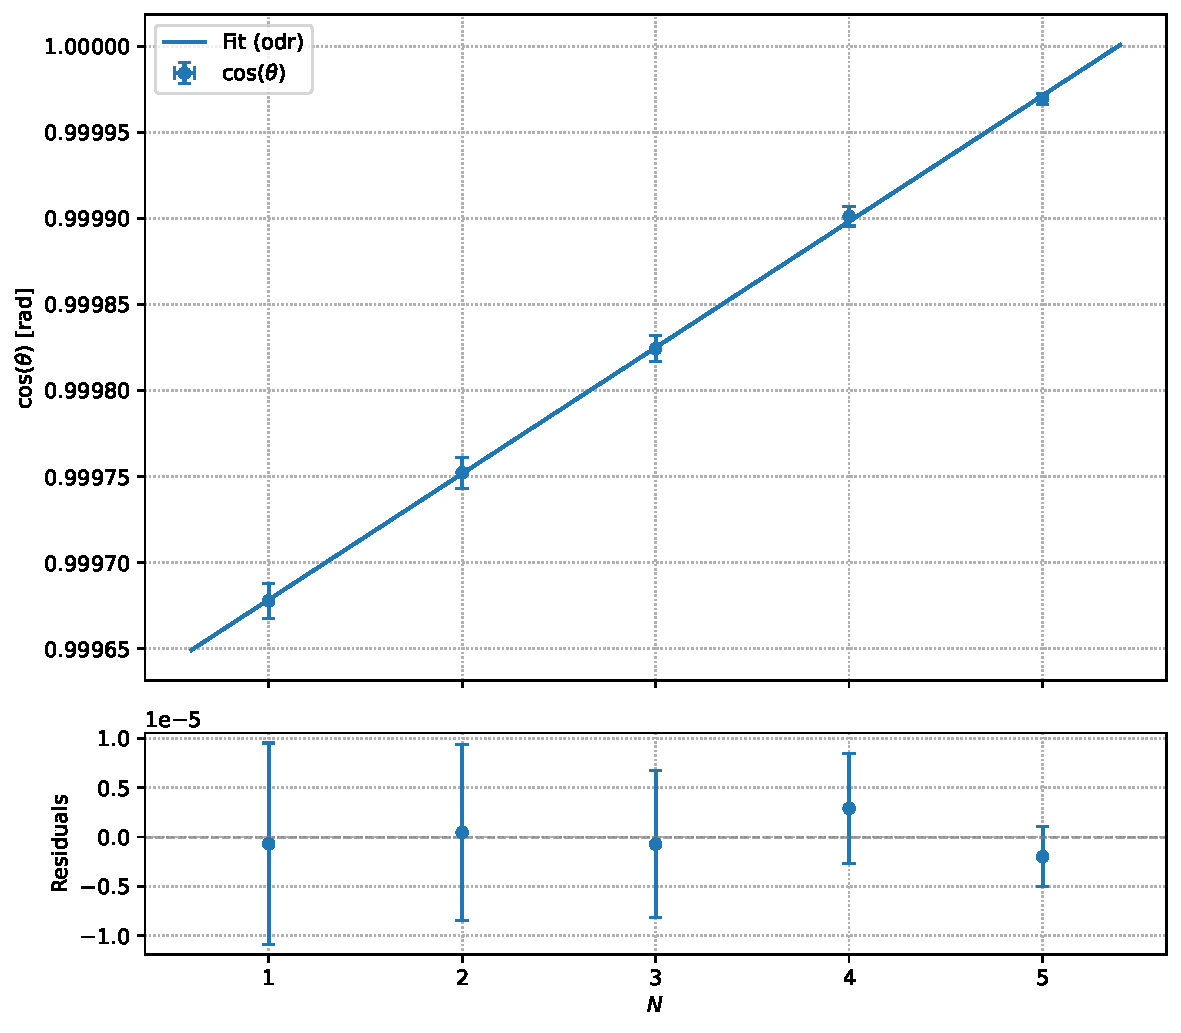
\includegraphics[width=1.0\textwidth]{./grafici/fabry_perot_interferenza.pdf}
\caption{Interpolazione della legge di Fabry-Perot}
\label{fig:fabry-perot-interpolazione}
\end{figure}

\begin{table}[htbp]
\centering
\begin{tabular}{|l|ccccc|}
\hline
Parametri & A & d & $\chi^2$ & DoF & $\chi^2/\nu$ \\\hline\hline
Risultati & \num{996.0 \pm 0.077 e-3} & $\SI{4.3 \pm 1.4}{\milli\meter}$ & \num{2.53e-3} & 3 & \num{8.42e-4} \\\hline
\end{tabular}
\caption{Risultati Interpolazione (Fabry-Perot)}
\label{tab:fabry-perot-risultati}
\end{table}

\subsection{Conclusioni}
Dall'interpolazione e dai risultati del test del chi quadro, visibili in tabella \ref{tab:fabry-perot-risultati}, si evince che la legge prevista è compatibile con l'osservazione sperimentale. Inoltre il valore di $d$, ampiezza della cavità, risulta coerente con quanto atteso. L'esperimento dimostra quindi che la condizione $\delta_r\frac{\lambda}{2\pi}+2d \cos \theta = N\lambda$ descrive accuratamente la posizione angolare dei massimi di interferenza nell'interferometro di Fabry-Perot. 

\section{Calibrazione micrometro con interferometro di Fabry-Perot}
\subsection{Obiettivo}
Verificare la calibrazione del nonio presente nella strumentazione attraverso lo studio della figura di interferenza prodotta su uno schermo.
Confrontare poi la precisione ottenuta sulle misure con quella garantita dal micrometro.
\subsection{Metodo}
Una volta montato e allineato l'interferometro, mantenendo la configurazione utilizzata per lo studio della figura di interferenza, abbiamo ruotato il 
nonio di una distanza fissa $d$, corrispondente all'allargamento della cavità di Fabry-Perot. Tale variazione della dimensione della cavità causa uno
scorrimento della figura di interferenza, in particolare dalla relazione \ref{eq: max interferenza fabry-perot} si può ricavare:
\begin{align}
    2 \Delta d \cos  \theta = \Delta N \lambda
\label{eq:calibrazione micrometro fabry-perot}
\end{align}
Fissata l'osservazione di un punto sulla figura di interferenza $\Delta N$ indica il numero di frange di cui si è osservato il passaggio attraverso quel punto, la lunghezza d'onda è $\lambda = 632.6 nm$ (come calcolato precedentemente) e $\theta$ rappresenta la posizione angolare a cui si trova il punto osservato, ossia l'angolo rispetto all'orizzontale di cui è inclinato il fascio.
Abbiamo variato le dimensioni della cavità 7 volte dello stesso tratto $d$ e per ciascuna di esse abbiamo misurato $\Delta N$, ricavando così 7 diversi valori di $\Delta d$, calcolato invertendo la relazione \ref{eq:calibrazione micrometro fabry-perot} come:
\begin{align}
    \Delta d = \frac{\lambda \Delta N}{2\cos{\theta}}
\label{eq:calibrazione micrometro fabry-perot invertita}
\end{align}

\subsection{Dati}
In tabella \ref{tab: micrometro fabry-perot} sono riportati i valori di $\Delta N$, ai quali è associata una sensibilità fissa $\delta_{\Delta N}$ pari ad 1 frangia, motivata dalla possibilità di errore umano nel conteggio del numero di frange osservate.

\begin{table}[htbp]
\centering
\caption{Shift di frangia osservato (interferometro di Fabry-Perot)}
\begin{tabular}{|l|ccccccc|}
\hline
Misura & 1 & 2 & 3 & 4 & 5 & 6 & 7 \\\hline\hline
$\Delta N$ & 24 ± 1 & 23 ± 1 & 23 ± 1 & 24 ± 1 & 25 ± 1 & 25 ± 1 & 23 ± 1 \\\hline
\end{tabular}
\label{tab: micrometro fabry-perot}
\end{table}

\subsection{Analisi dati}
Dal momento che l'angolo $\theta$ è molto piccolo nel ricavare $\Delta d$ è stata utilizzata l'approssimazione $\cos{\theta}\approx1$ da cui consegue:
\begin{align}
    \Delta d_{approx} = \frac{\lambda \Delta N}{2}
\label{eq:calibrazione micrometro fabry-perot invertita}
\end{align}
L'imprecisione introdotta da tale considerazione è stata valutata considerando il minimo valore di $\cos{\theta}$, ossia quello che più si discosta dall'approssimazione $\cos{\theta}\approx1$, precedentemente misurato. Per quanto mostrato in tabella \ref{tab:fabry-perot-dati} tale valore risulta $\cos_{min}=0.99968$.
Abbiamo quindi sostituito $\cos_{min}$ a 1 e osservato la variazione di $\Delta d_{approx}$ rispetto a $\Delta d$ ottenendo: $\Delta d_{approx} = 0.99968\Delta_d$. L'approssimazione utilizzata introduce quindi un'incertezza relativa $\frac{\Delta d- \Delta d_{approx}}{\Delta d}=\sigma_{\Delta d}=0.03\%$, da confrontare poi con l'errore sul valore di $\Delta d$.
L'errore sull'allargamento della cavità di Fabry-Perot è determinato propagando gli errori rispetto alla relazione \ref{eq:calibrazione micrometro fabry-perot invertita}, ricavando quindi:
\begin{align}
   \sigma_{\Delta d}= \frac{\lambda \delta_{\Delta N}}{2}
\label{eq:errore calibrazione micrometro fabry}
\end{align}
Quanto calcolato dalle relazioni \ref{eq:calibrazione micrometro fabry-perot invertita} e \ref{eq:errore calibrazione micrometro fabry} è visualizzabile in tabella \ref{tab: distanze calibrazione fabry-perot}.
\begin{table}[htbp]
\centering
\caption{Distanze calibrazione micrometro (interferometro di Fabry-Perot)}
\begin{tabular}{|l|ccccccc|}
\hline
Misura & 1 & 2 & 3 & 4 & 5 & 6 & 7 \\\hline\hline
$\Delta d [\mu m]$ & 7.6 ± 0.3  & 7.3 ± 0.3  & 7.3 ± 0.3  & 7.6 ± 0.3  & 7.9 ± 0.3 & 7.9 ± 0.3 & 7.3 ± 0.3 \\\hline
\end{tabular}
\label{tab: distanze calibrazione fabry-perot}
\end{table}
Come si può osservare l'errore relativo introdotto dalla sensibilità di misura risulta molto maggiore di $\sigma_{\Delta d}$; l'approssimazione ad 1 di $\cos{\theta}$ è quindi lecita.

\subsection{Conclusione}
Per ricavare la migliore stima di $\Delta_d$ e per ridurne l'incertezza abbiamo calcolato la media tra i valori presenti in tabella \ref{tab: distanze calibrazione fabry-perot}, ottenendo $\Delta d_{best} = (7.5 \pm 0.1) \mu m$. Possiamo quindi concludere come l'utilizzo dell'interferometro ci abbia permesso di misurare distanze con una precisione pari a $0.1 \mu m$, dieci volte superiore rispetto alla sensibilità del micrometro.


\section{Calibrazione micrometro con interferometro di Michelson}
\subsection{Obiettivo}
L'obiettivo di questa esperienza è la calibrazione del micrometro mediante l'utilizzo di un interferometro nella configurazione di Michelson. In particolare si vuole dimostrare che la sensibilità del micrometro è inferiore alla precisione ricavata mediante l'utilizzo delle formule riguardanti l'interferenza, ovvero che la misura indiretta dello spostamento dello specchio mediante il conteggio delle frange è più precisa della misura diretta.
\subsection{Metodo}
Per effettuare le misure è stato creato un interferometro di Michelson la cui rappresentazione schematica è riportata nell'immagine \ref{Fig: Configurazione Michaelson}:
\begin{center}
	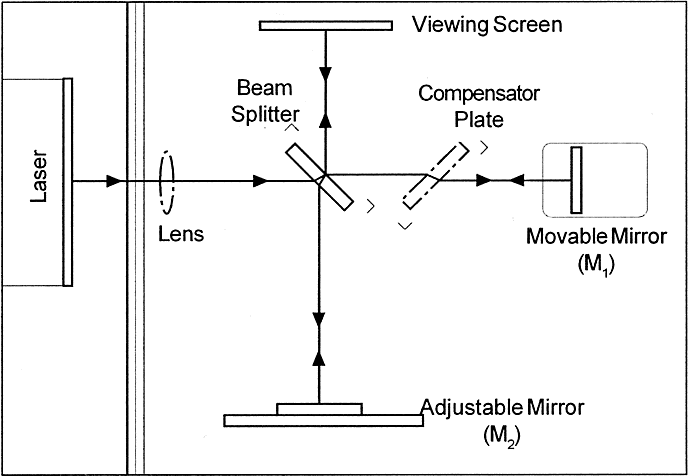
\includegraphics[width=0.9\textwidth]{./grafici/configurazione michaelson.png}
\captionof{figure}{Configurazione interferometro Michelson (da manuale PASCO)}
\label{Fig: Configurazione Michaelson}
\end{center}
L'interferometro è composto da un laser che invia un raggio luminoso ad una lente divergente, la quale rende i raggi della sorgente paralleli fra di loro. Il raggio collimato incide poi su uno specchio semi-riflettente creando così due diversi fasci che compiono percorsi separati per poi incontrarsi nuovamente su uno schermo. I diversi raggi incidenti compiono cammini ottici differenti (percorrono distanze diverse), quindi quando incidono sullo schermo creano una figura di interferenza. Tale figura è osservabile a occhio nudo e si presenta come un'alternanza di cerchi concentrici; ciascun cerchio rappresenta una regione di interferenza costruttiva. Variando la posizione dello specchio mobile è possibile cambiare anche il cammino ottico dei due raggi e dunque osservare uno shift della figura di interferenza. In tal caso si osserverà un'alternanza di frange concentriche il cui numero varierà secondo la relazione: 
\begin{center}
    $2 \Delta d=\Delta N \lambda $
\end{center}
dove $\Delta d$ è lo spostamento dello specchio, $\Delta N$ è il numero di frange che si alternano ad una data posizione e $\lambda=632.6 nm$ è la lunghezza d'onda del fascio incidente ed è considerabile valore noto. Lo spostamento dello specchio mobile è possibile grazie all'apparato, il quale consente di variarne la posizione mediante un nonio con scala graduata di precisione $1 \mu m$. Il conteggio dei massimi della figura di interferenza è stato effettuato manualmente, variando la posizione dello specchio mobile e contando ad occhio le frange.
\subsection{Dati}
Nella tabella \ref{tab: micrometro Michaelson} sono riportati i valori di $\Delta N$ contati in laboratorio per ciascuna delle 7 misure effettuate. Per effettuare tale misura abbiamo variato la posizione dello specchio di un valore costante tramite il micrometro sull'apparato e abbiamo contato il relativo numero di frange che si alternavano sullo schermo. L'errore sul numero di frange contate associato a ciascun valore è di $\pm1$ ed è motivato dal fatto che le frange si devono presentare in valori discreti e dal fatto che il conteggio è stato effettuato manualmente. 
\begin{table}[htbp]
\centering
\caption{Shift di frangia osservato (interferometro di Michelson)}
\begin{tabular}{|l|ccccccc|}
\hline
Misura & 1 & 2 & 3 & 4 & 5 & 6 & 7 \\\hline\hline
$\Delta N$ & 23 ± 1 & 25 ± 1 & 26 ± 1 & 23 ± 1 & 26 ± 1 & 24 ± 1 & 24 ± 1 \\\hline
\end{tabular}
\label{tab: micrometro Michaelson}
\end{table}
\subsection{Analisi dati}
A partire dai dati raccolti siamo riusciti a calcolare il valore di $d$ atteso tramite la formula: 
\begin{center}
    $\Delta d=\frac{\Delta N \lambda}{2}$
\end{center}
Otteniamo così vari valori di $d$ i quali sono riportati nella tabella \ref{tab: valori d michaelson}:
\begin{table}[htbp]
\centering
\caption{Valore di d calcolato}
\begin{tabular}{|l|ccccccc|}
\hline
Misura & 1 & 2 & 3 & 4 & 5 & 6 & 7 \\\hline\hline
$\Delta d(\mu m)$ & 7.3 ± 0.3 & 7.9 ± 0.3 & 8.2 ± 0.3 & 7.3 ± 0.3 & 8.2 ± 0.3 & 7.6 ± 0.3 & 7.6 ± 0.3 \\\hline
\end{tabular}
\label{tab: valori d michaelson}
\end{table} 
Il valore di $d$ finale è stato poi considerato come la media dei vari valori di $d$ ricavati. Otteniamo così $\Delta d_{best}=(7.7\pm0.1 )\mu m$.
Siccome i valori degli spostamenti dello specchio mobile per gli esperimenti di Fabry-Perot e di Michelson sono uguali in quanto abbiamo ruotato il nonio in modo identico nel corso delle misurazioni, ci aspettiamo compatibilità tra i valori di $\Delta d$ ottenuti nelle due configurazioni. Abbiamo quindi effettuato il t-test con $t=\frac{|\Delta d_{Michaelson}-\Delta d_{Fabry-Perot}|}{\sqrt{2\sigma^2}}$=1.42, il quale equivale a una probabilità entro t-sigma $p=0,84$
\subsection{Conclusioni}
Innanzitutto possiamo osservare che i valori di $\Delta d$ sono compatibili fra di loro, inoltre la sensibilità ottenuta mediante la misura indiretta di $\Delta d$, ricavata osservando il passaggio di frange, risulta notevolmente maggiore rispetto a quella del micrometro, dunque l'utilizzo dell'interferometro ha permesso di misurare distanze in modo più preciso.

\section{Misura dell'indice di rifrazione dell'aria}
\subsection{Obiettivo}
Stimare l'indice di rifrazione dell'aria e valutare la sua dipendenza dalla pressione osservando la figura di interferenza prodotta dall'interferometro di Michelson.

\subsection{Metodo}
Mantenendo la stessa configurazione precedente è stata montata tra lo specchio semi-riflettente e lo specchio mobile una cella a vuoto la cui pressione poteva essere regolata utilizzando un manometro. Dal momento che il cammino ottico $D$ percorso dalla luce all'interno della cella dipende dall'indice di rifrazione del mezzo secondo la relazione $D=nd$, con $d$ spessore della cella, variando $n$ si può causare una variazione di cammino ottico $\Delta D$. Sappiamo poi che l'indice di rifrazione dell'aria dipende dalla sua pressione $P$ in modo lineare, vale cioè: 
\begin{align}
    n(P) = 1 + mP 
\end{align}
Ne consegue che ad una variazione di pressione seguirà una variazione del cammino ottico percorso dalla luce e di conseguenza un cambiamento nella figura di interferenza prodotta. Più precisamente diminuendo la pressione si avrà uno shift di frange dovuto dal fatto che la radiazione deve compiere un percorso minore, esso diminuisce infatti di $\Delta D= 2d \Delta n= 2dm(P_f-P_i)$. \footnote{Il fattore 2 è dovuto dal fatto che la luce passa due volte attraverso la cella a vuoto in quanto viene riflessa dallo specchio} 
Si ha quindi che è possibile osservare il passaggio attraverso un punto sullo schermo di $\Delta N$ frange, dove $\Delta N$ soddisfa la relazione:
\begin{align}
    \Delta N \lambda= 2dm(P_f-P_i)
\label{eq: shift frange pressione aria}
\end{align}
Abbiamo quindi proceduto variando più volte la pressione all'interno della cella mediante la pompa collegata al manometro, e contando il numero di frange che passavano sullo schermo in un punto fissato.

\subsection{Dati}
Abbiamo considerato noti i valori di $\lambda=632.6 nm$ lunghezza d'onda del laser e $d=3 cm$ spessore della cella. I valori di $\Delta P$ e $\Delta N$ misurati sono invece raccolti in tabella \ref{tab: delta p e delta n}. Per quanto riguarda le pressioni esse corrispondono a quanto osservato sul manometro, indicano quindi la variazione $P_f- P_i$ rispetto alla pressione atmosferica ($P_i = 100 kPa$). L'incertezza $\delta_{\Delta P}$ è stata considerata pari alla sensibilità di misura, quindi $\delta_{\Delta P}=2 kPa$; mentre, come nelle esperienze precedenti, abbiamo valutato l'errore sul conteggio dello shift di frange pari ad 1 frangia.

\begin{table}[htbp]
\centering
\caption{Variazioni di pressione e shift di frange}
\label{tab: delta p e delta n}
\begin{tabular}{|l|ccccccc|}
\hline
Misura & 1 & 2 & 3 & 4 & 5 & 6 & 7 \\\hline\hline
$\Delta P [kPa]$ & 10 ± 2 & 20 ± 2 & 30 ± 2 & 40 ± 2 & 50 ± 2 & 60 ± 2 & 70 ± 2 \\\hline
$\Delta N$ & 3 ± 1 & 6 ± 1 & 9 ± 1 & 12 ± 1 & 15 ± 1 & 18 ± 1 & 21 ± 1 \\\hline
\end{tabular}
\end{table}

\subsection{Analisi dati}
Invertendo la relazione \ref{eq: shift frange pressione aria} abbiamo ottenuto:
\begin{align}
    \Delta N = \frac{2dm \Delta P}{\lambda}
\end{align}

\begin{figure}[htbp]
\centering
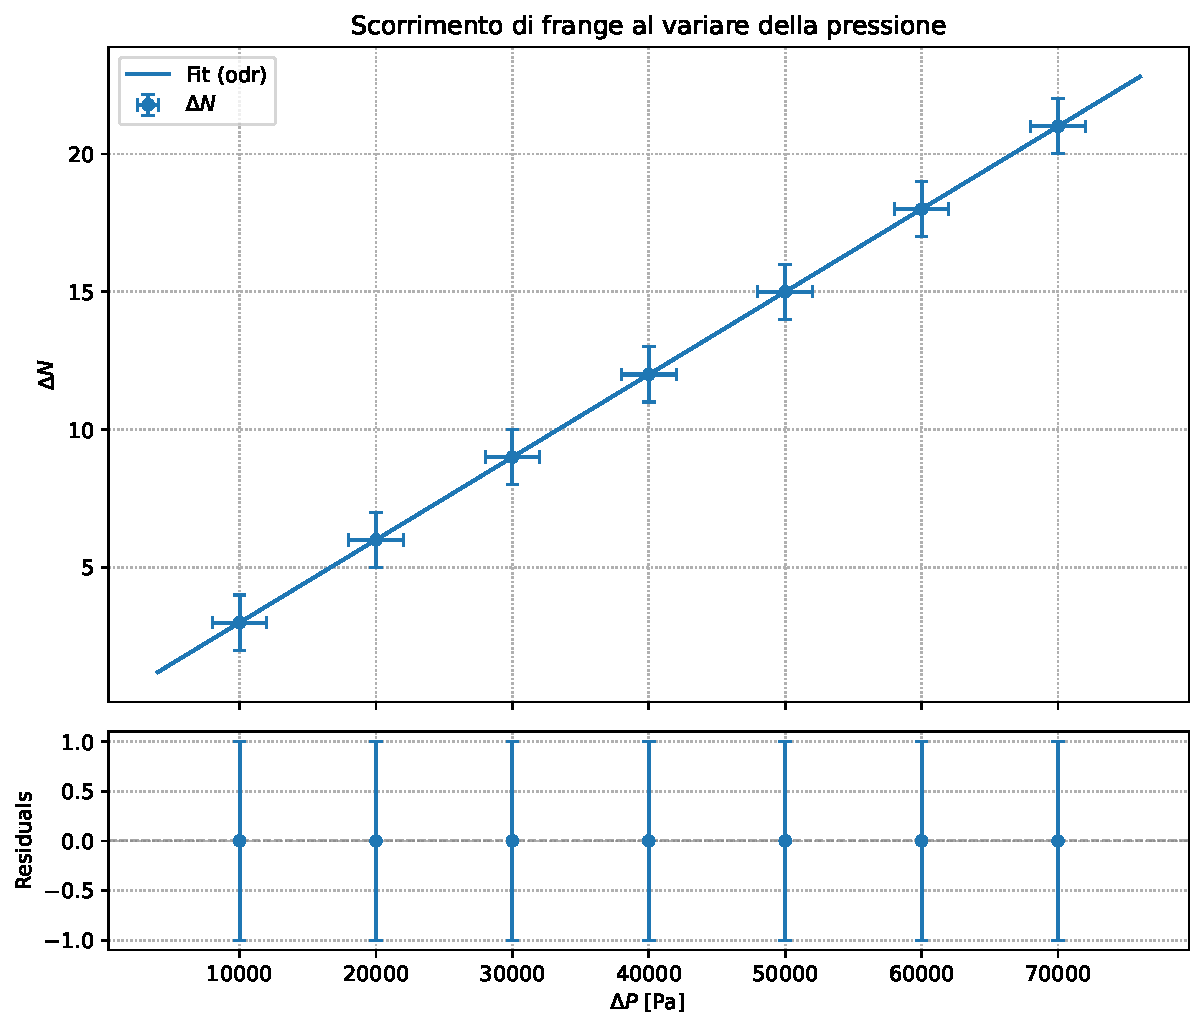
\includegraphics[width=1.0\textwidth]{./grafici/indice_aria.pdf}
\caption{Relazione shift di frange-variazione di pressione}
\label{fig: indice aria}
\end{figure}

Tale relazione, la quale lega linearmente $\Delta N$ e $\Delta P$, come è possibile osservare in figura \ref{fig: indice aria}, è stata utilizzata per realizzare un'interpolazione lineare, mirata ad ottenere la migliore stima del parametro $m$.
Quanto ricavato dall'interpolazione e i risultati del suo test del chi quadro è visibile in tabella \ref{tab: fit indice rifrazione aria}.

\begin{table}[htbp]
\centering
\caption{Risultati fit indice di rifrazione aria}
\label{tab: fit indice rifrazione aria}
\begin{tabular}{|l|cccc|}
\hline
Fit & m [1/kPa] & $\chi^2$ & DoF & $\chi^2/\nu$ \\\hline\hline
Risultati & 3.16 ± 0.10 n & 0 & 6 & 0 \\\hline
\end{tabular}
\end{table}

Stimato $m_s$ abbiamo poi ricavato l'indice di rifrazione dell'aria a pressione atmosferica ($P_{atm}= 101.325 kPa$) come:
$n_s = 1+m_sP_{atm}$ con errore $\delta_n = \delta_{m_s}P_{atm}$, ottenendo $n_s =1.00032 \pm 0.00001$.

\subsection{Conclusione}
Come è possibile osservare dall'esito estremamente favorevole del test del chi quadro, riportato in tabella \ref{tab: fit indice rifrazione aria}, possiamo considerare il fit realizzato in accordo con i dati sperimentali. Abbiamo poi osservato come aver ottenuto un valore di $\chi^2/\nu$ nullo non sia da attribuirsi ad errori sovrastimati, infatti anche diminuendo l'errore sui valori di $\Delta N$ e $\Delta P$ si otterrebbe $\chi^2/\nu= 0$, data la completa esattezza. Infine abbiamo confrontato l'indice di rifrazione ricavato sperimentalmente con quello atteso per una temperatura di 25$^\circ$ (pari circa a quella del laboratorio): $n_{att} =1.00029$. Abbiamo utilizzato come test di compatibilità il t-test ottenendo $t= \frac{n_s-n_{att}}{\delta_{n_s}}=3$, esito al quale corrisponde p-value=0. Tale incompatibilità può essere attribuita alla dipendenza dell'indice di rifrazione dell'aria dalla temperatura. Seppur questa dipendenza sia minima essa può causare una variazione di $n_{att}$ coerente con lo scostamento $n_s-n_{att}$.

\section{Misura dell'indice di rifrazione del vetro}
\subsection{Obiettivo}
L'obiettivo di questa esperienza è la misura dell'indice di rifrazione del vetro di un  piccolo schermo mediante l'utilizzo di un interferometro di Michaelson.
\subsection{Metodo}
Per effettuare le misure è stato creato un interferometro di Michaelson (descritto precedentemente) all'interno del quale è stata posizionata una lastra di vetro inclinabile come nell'immagine \ref{Fig: Configurazione Michaelson vetro}:
\begin{center}
	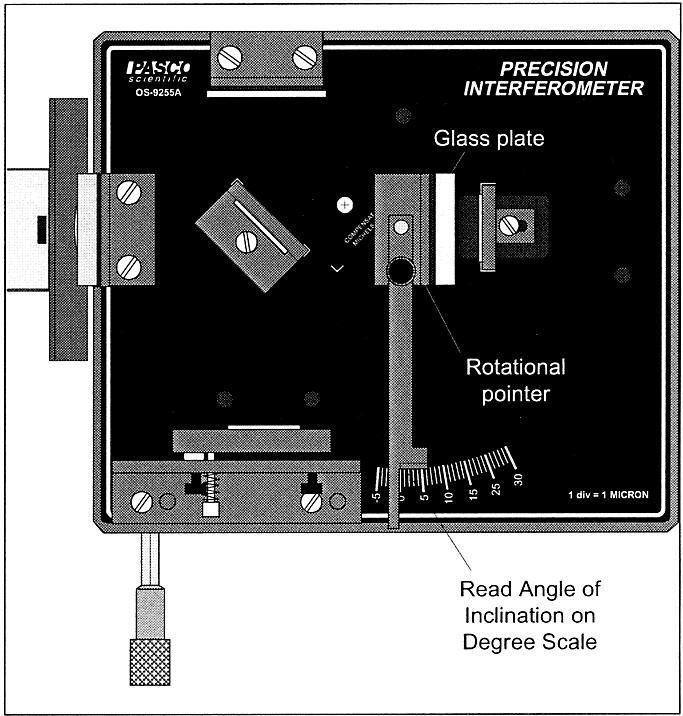
\includegraphics[width=0.9\textwidth]{./grafici/Michaelson vetro.png}
\captionof{figure}{Configurazione interferometro Michaelson con lastra di vetro (da manuale PASCO)}
\label{Fig: Configurazione Michaelson vetro}
\end{center}
La lastra di vetro inclinabile è attaccata ad un'asta di metallo che permette di leggere l'angolo di inclinazione su di una scala graduata. Abbiamo dunque osservato lo shift di frange, campionando $\Delta N$ in funzione dell'angolo di inclinazione della lastra $\theta$. Osserviamo che vi era un angolo di inversione in prossimità del quale le frange cambiavano direzione. Abbiamo dunque deciso di campionare angoli maggiori dell'angolo di inversione per evitare problemi con l'applicazione delle formule. In particolare abbiamo iniziato a misurare gli angoli proprio a partire dall'angolo di minima deviazione, il quale si trovava ad un angolo di $\theta_i = (0\pm 0.2)^\circ$ rispetto al goniometro; la misura dell'angolo finale sarà dunque equivalente al valore letto sul goniometro, tale considerazione influisce unicamente sull'errore. L'errore sull'angolo iniziale è dovuto allo spessore delle linee e dal fatto che fosse difficile individuare il punto preciso in cui le linee cominciavano a muoversi, sia a causa della sensibilità dello strumento sia a causa dello spessore delle linee stesse.La relazione che lega l'indice di rifrazione del vetro all'angolo di inclinazione e al numero di frange è la seguente:
\begin{center}
    $n_{\text{vetro}} = \frac{(2d - \Delta N \lambda)(1 - \cos\theta)}{2d(1 - \cos\theta) - \Delta N \lambda}$
\label{eq:indice rifrazione vetro}
\end{center}
dove d è lo spessore della lastra di vetro e $\lambda=632.6nm$ è la lunghezza d'onda del laser in aria, valore noto.
Come prima la misura di $\Delta N$ è stata effettuata contando l'alternanza di frange ad occhio.
\subsection{Dati}
Nella tabella \ref{tab: valori michaelson vetro} sono riportati i valori di $\Delta N$ osservati in laboratorio ed il relativo angolo di inclinazione $\theta$ rispetto all'angolo di minima deviazione. L'angolo $\theta$ è stato calcolato come $\theta = \theta_f - \theta_i$, operazione che non ha effetti sul valore dell'angolo ma solo sulla sua incertezza.

\begin{table}[htbp]
\centering
\begin{tabular}{|l|ccccc|}
\hline
Label & 1 & 2 & 3 & 4 & 5 \\\hline\hline
$\theta_f(^\circ)$ & 2.0 ± 0.1 & 4.0 ± 0.1 & 6.0 ± 0.1 & 8.0 ± 0.1 & 10.0 ± 0.1 \\\hline
$\theta(^\circ)$ & 2.0 ± 0.2 & 4.0 ± 0.2 & 6.0 ± 0.2 & 8.0 ± 0.2 & 10.0 ± 0.2 \\\hline
$\Delta N$ & 3 ± 1 & 13 ± 1 & 26 ± 1 & 58 ± 2 & 87 ± 3 \\\hline
\end{tabular}
\end{table}

Il conteggio di $\Delta N$ è stato effettuato da 2 persone contemporaneamente, al fine di minimizzare l'errore umano. In tabella sono state riportate le medie del numero di frange da loro contate e come errore è stata scelta la semi-dispersione dei due valori di $\Delta N$ misurati o 1 in caso tale valore fosse $<1$; l'errore su $\theta$ è la sensibilità del goniometro. Invece lo spessore della lastra di vetro è stato considerato noto, cioè $d=(6.8 \pm 0.1)mm$, come indicato sulla scheda PASCO.
\subsection{Analisi dati}
A partire dai dati raccolti abbiamo calcolato l'indice di rifrazione del vetro per ciascuna coppia di dati, i vari valori di $n_{vetro}$ ottenuti dalla relazione \ref{eq:indice rifrazione vetro} sono riportati nella tabella \ref{tab:indice_rifrazione_vetro}. L'errore $\delta_{n_{vetro}}$ è stato ricavato applicando la propagazione degli errori alla relazione \ref{eq:indice rifrazione vetro} rispetto all'incertezza su $\Delta N$ e $d$.
\begin{table}[h!]
\centering
\begin{tabular}{|c|c|}
\hline
\textbf{Misura} & \( n_{\text{vetro}} \) \\
\hline
1 & \( 1.3 \pm 0.5 \) \\
2 & \( 1.3 \pm 0.3 \) \\
3 & \( 1.3 \pm 0.2 \) \\
4 & \( 1.4 \pm 0.1 \) \\
5 & \( 1.4 \pm 0.1 \) \\
\hline
\end{tabular}
\caption{Indice rifrazione vetro}
\label{tab:indice_rifrazione_vetro}
\end{table}
L'indice di rifrazione del vetro è stato infine valutato come media dei vari valori ottenuti, così da ridurne l'incertezza relativa. Abbiamo ricavato:
\begin{center}
    $n_{vetro}=1.34 \pm 0.07$
\end{center}
\subsection{Conclusioni}
Non conoscendo in maniera esatta l'indice di rifrazione della lastra di vetro presente in laboratorio non possiamo affermare nulla riguardo alla compatibilità del valore trovato. Tuttavia, in generale, i vari tipi di vetro presentano un indice di rifrazione superiore a $1.5$, che è superiore a quello da noi calcolato. In conclusione l'indice di rifrazione trovato non sembra essere compatibile con il valore atteso di $n>1.5$. 
\section{Interferenza con un righello}
\subsection{Obiettivo}
Stimare la lunghezza d'onda $\lambda$ di un laser attraverso l'analisi della figura di interferenza prodotta dall'illuminazione obliqua di un righello. 

\subsection{Metodo}
Quando un fascio laser monocromatico e coerente incide obliquamente su un righello metallico dotato di incisioni regolari, si verificano fenomeni di diffrazione ai bordi delle tacche che agiscono come un reticolo di diffrazione. La relazione che descrive la posizione dei massimi di interferenza in questa configurazione è: 
\begin{align}
    d(\cos\theta_i - \cos\theta_N) = N\lambda
\end{align}
dove $d=\SI{1}{\milli\meter}$ è il passo del reticolo, in questo caso la distanza tra le incisioni del righello, $\theta_i$ è l'angolo di incidenza del fascio laser, $\theta_N$ è l'angolo corrispondente al massimo di ordine $N$, e $\lambda$ è la lunghezza d'onda del laser, stimato come $\lambda=\SI{632.8}{\nano\meter}$ per il laser He-Ne utilizzato.

La distanza tra la parete e il punto di riflessione del laser sul righello è stato stimato come $L=\SI{124 \pm 5}{\centi\meter}$, il motivo di un'incertezza così alta è dovuto al fatto che non è stato possibile individuare con precisione il punto di riflessione corrispondente al primo massimo. Il righello presentava una "striscia" di punti di diffrazione, tuttavia questa incertezza, come si vedrà dall'analisi dati, non ha un impatto significativo sul risultato finale. $\theta_i$ è stato dunque calcolato con $L$ e la distanza tra l'immagine del raggio indeflesso e di quello riflesso, $r$, con la seguente relazione:
\begin{align}   
    \theta_i = \arctan\left(\frac{r}{L}\right)
\end{align}
similmente $\theta_N$ è stato calcolato come:
\begin{align}
    \theta_N = \arctan\left(\frac{r_N}{L}\right)
\end{align}
dove $r_N$ è la distanza tra l'immagine del raggio indeflesso e di quello riflesso per il massimo di ordine $N$.
\subsection{Dati}
È stato misurato $r=\SI{4.7 \pm 0.2}{\centi\meter}$, da cui $\theta_i=\SI{0.038 \pm 0.002}{\radian}$, le misure di $r_N$ per i vari massimi sono riportate in \cref{tab:interferenza-righello}, insieme agli altri dati.

\begin{table}[htbp]
\caption{Dati della figura di interferenza (righello)}
\label{tab:interferenza-righello}
\centering
\begin{tabular}{|l|ccccc|}
\hline
Label & 1 & 2 & 3 & 4 & 5 \\\hline\hline
$r_N$ [\si{\milli\meter}]& \num{70 \pm 2} & \num{85 \pm 2} & \num{96 \pm 2} & \num{110 \pm 2} & \num{120 \pm 2} \\\hline
$\cos(\theta_i) - \cos(\theta_N)$ [\num{e-6}]& \num{0.872 \pm 0.200} & \num{1.6 \pm 0.2} & \num{2.3 \pm 0.3} & \num{3.2 \pm 0.4} & \num{3.9 \pm 0.4} \\\hline
$N$ & 1 & 2 & 3 & 4 & 5 \\\hline
\end{tabular}
\end{table}

\subsection{Analisi dati}
L'interpolazione
\begin{align}
    (\cos\theta_i - \cos\theta_N) = \frac{N\lambda}{d}
\end{align}
è riportata in \cref{fig:interferenza-righello-interpolazione}, i risultati sono riportati in \cref{tab:interferenza-righello-risultati}.

\begin{figure}[htbp]
\centering
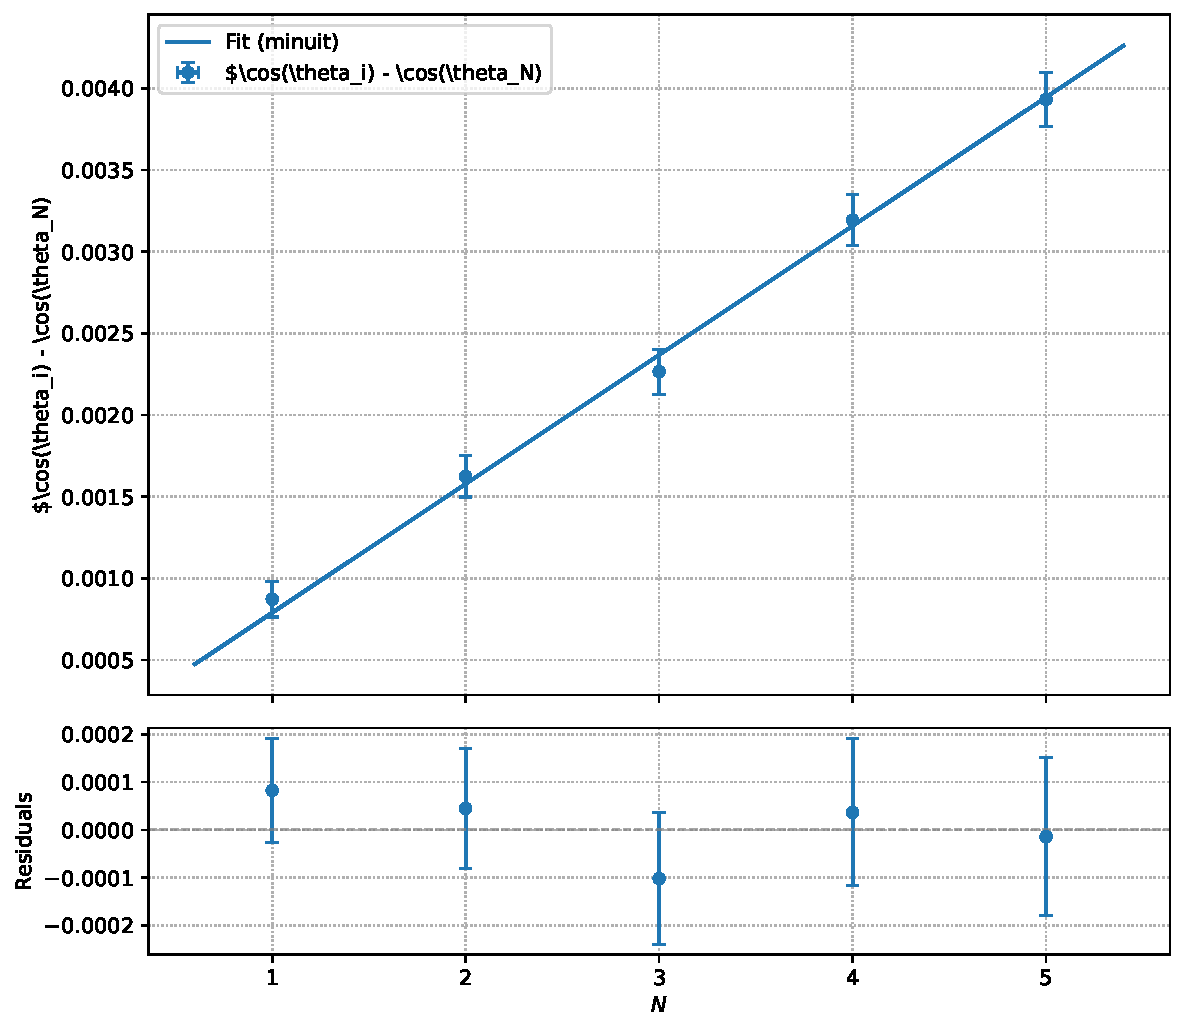
\includegraphics[width=1.0\textwidth]{./grafici/righello.pdf}
\caption{Interpolazione della legge di interferenza (righello)}
\label{fig:interferenza-righello-interpolazione}
\end{figure}

\begin{table}[htbp]
\caption{Risultati del Fit - Interferenza del Righello}
\label{tab:interferenza-righello-risultati}
\centering
\begin{tabular}{|l|cccc|}
\hline
parametri & $\lambda$ & $\chi^2$ & DoF & $\chi^2/\nu$ \\\hline\hline
fit (minuit) & \SI{792 \pm 45}{\nano\meter} & \num{0.393} & 4 & \num{0.0983} \\\hline
\end{tabular}
\end{table}

\subsection{Conclusioni}
La lunghezza d'onda stimata è $\lambda = \SI{792 \pm 45}{\nano\meter}$, che è incompatibile con il valore noto di $\lambda = \SI{632.8}{\nano\meter}$ per il laser He-Ne ($\approx \num{3.5} \sigma$, p-value = \num{0.0001}). Il fit, avendo un chi quadro ridotto, suggerisce che la legge usata descriva correttamente il fenomeno, dal punto di vista della relazione lineare tra $\cos(\theta_i) - \cos(\theta_N)$ e $N$, e la grossa incertezza sulla misura di $L$ non compromette questo risultato, infatti ipotizzando un errore del millimetro risulterebbe comunque un chi quadro ridotto di \num{0.328}. Ipotizziamo dunque che la legge racchiuda correttamente la fisica dietro il fenomeno, ma manchi di qualche fattore correttivo dovuto alla non idealità del sistema. 
\end{document}